\documentclass[tikz,border=6pt]{standalone}
\usepackage[T1]{fontenc}
\usepackage[utf8]{inputenc}
\usepackage{pgfplots}
\pgfplotsset{compat=1.18}
\begin{document}
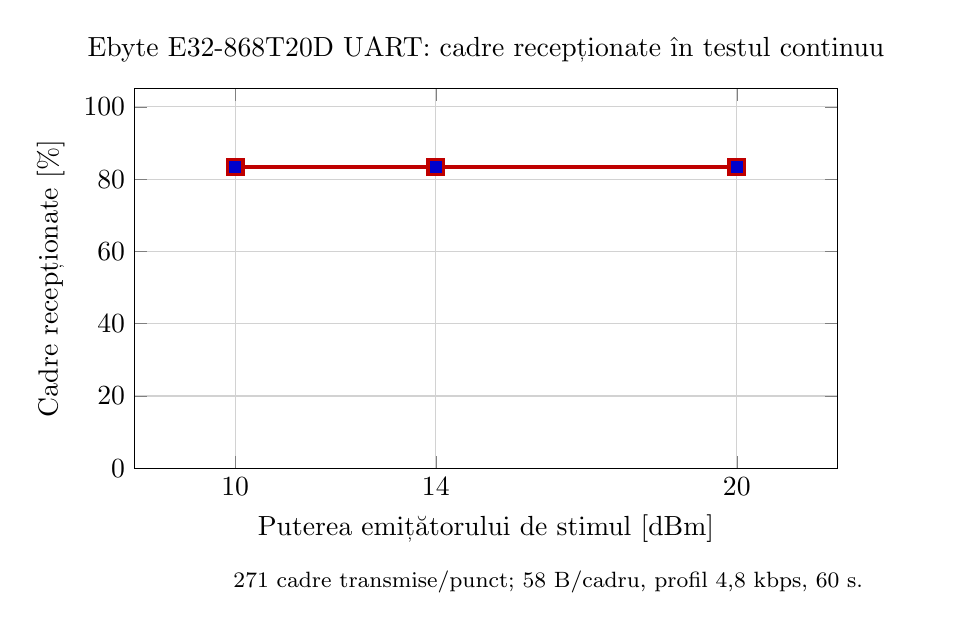
\begin{tikzpicture}
\begin{axis}[width=10.5cm, height=6.4cm,
  title={Ebyte E32-868T20D UART: cadre recepționate în testul continuu},
  xmin=8, xmax=22, xtick={10,14,20},
  ymin=0, ymax=105, ytick={0,20,40,60,80,100},
  xlabel={Puterea emițătorului de stimul [dBm]},
  ylabel={Cadre recepționate [\%]},
  grid=both, minor grid style={gray!15}, major grid style={gray!35},
]
\addplot+[red!75!black, line width=1.2pt, mark=square*, mark size=2.8pt] coordinates {(10,83.3948339) (14,83.3948339) (20,83.3948339)};
\end{axis}
\node[font=\footnotesize, align=center, text width=10cm] at (5.25,-1.45)
  {271 cadre transmise/punct; 58 B/cadru, profil 4{,}8 kbps, 60 s.};
\end{tikzpicture}
\end{document}
